% Provenance (never printed): see sources/outline_sources.md (Year 3: Gibbs
% energy and the phase rule in rocks, chemical potential recalled from the
% chemistry book; ternary diagrams; pseudosections, principle). Brief:
% sources/book5/BRIEFS.md, ch. 11. Curves from figdata/bachelor-3/
% gasp_tables.py, schreinemakers.py and regular_solution.py. Exercise and
% problem values in the Book 5 scratch calculator calc/ch11.py.
\chapter{岩石热力学}\label{ch:b3:petrological-thermodynamics}

一颗几毫米宽的石榴子石，随其片岩被埋深、加热而逐层生长。
它的边缘仍记录着钙、铁、镁的含量，
即它最后与周围黑云母和斜长石达到的平衡。第二学年分册
用两个经过标定的方程，把这类成分换算为温度与压强。
本章打开这一“盒子”：这些方程从何而来，实测焓与熵的表格
可信到何种程度，一种岩石能含多少种矿物，
固溶体如何混合与分离，
以及计算机如何把体系的总成分转换为
应当出现的组合图。

\begin{recall}
吉布斯能、化学势、活度与平衡常数、
方差与相律、互溶间隙与杠杆规则，
均见化学书的大学分册。单变反应、
其克拉珀龙斜率 $\Delta_rS/\Delta_rV$、不变点，以及
由表格算出的铝硅酸盐图，见第二学年分册中
关于变质相的一章；地质温度计与地质压力计、
石榴子石–黑云母交换温度计与 GASP 压力计，见其中
关于 P--T--t 轨迹的一章；三元图与共结线，见其中关于岩浆的一章。
固溶体及其端元，见第一学年分册中
关于矿物的一章。
\end{recall}

\section{由表格求平衡}\label{sec:b3:petrological-thermodynamics:tables}

对于成分固定的矿物之间的反应，
其在温度 $T$、压强 $P$ 下的平衡条件为 $\Delta_rG(T, P) = 0$。表格给出
\qty{298.15}{K}、\qty{1}{bar} 下各矿物的生成焓、熵与摩尔体积，
以及以上的热容 $C_p(T)$。第二学年分册
取 $\Delta_rH$、$\Delta_rS$ 与 $\Delta_rV$ 为常数。
一般结果如下。

\begin{theorem}[$T$ 与 $P$ 下反应的吉布斯能]\label{thm:b3:petrological-thermodynamics:dg}
设一反应在 $T_0 = \qty{298.15}{K}$、\qty{1}{bar} 下，
其焓变为 $\Delta_rH^\circ$，熵变为 $\Delta_rS^\circ$，热容变化为 $\Delta_rC_p(T)$；
对于固体，体积变化 $\Delta_rV$
与 $T$、$P$ 无关。则
\[
  \Delta_rG(T, P) = \Delta_rH^\circ + \int_{T_0}^{T}\Delta_rC_p\,\mathrm dT
  - T\Bigl(\Delta_rS^\circ + \int_{T_0}^{T}\frac{\Delta_rC_p}{T}\,\mathrm dT\Bigr)
  + (P - 1)\,\Delta_rV ,
\]
平衡线为 $P = 1 - \Delta_rG(T, 1)/\Delta_rV$。
\end{theorem}

\begin{proof}
在 \qty{1}{bar} 下，$(\partial\Delta_rH/\partial T)_P = \Delta_rC_p$ 且
$(\partial\Delta_rS/\partial T)_P = \Delta_rC_p/T$；从 $T_0$ 积分，
得 $\Delta_rH(T)$ 与 $\Delta_rS(T)$，且 $\Delta_rG = \Delta_rH -
T\Delta_rS$。固定 $T$ 时，$(\partial\Delta_rG/\partial P)_T = \Delta_rV$，
由假设为常数；从 1 积分到 $P$，得附加项 $(P - 1)\Delta_rV$。
令 $\Delta_rG(T, P) = 0$，即得平衡线。
\end{proof}

两个积分部分抵消：其和为 $\int_{T_0}^T\Delta_rC_p(1 -
T/T')\,\mathrm dT'$，其中因子 $1 - T/T'$ 为负，
且在 $T'$ 接近 $T$ 时数值很小。对于固体，$\Delta_rC_p$ 本身很小，
因为矿物的热容近似等于其各氧化物热容之和。
因此常数近似是良好的，表格可以说明其好到何种程度。
对于 GASP 反应，
\[
  \ce{3 CaAl2Si2O8 <=> Ca3Al2Si3O12 + 2 Al2SiO5 + SiO2},
\]
汇总表给出 $\Delta_rH^\circ = \qty{-36.3}{kJ}$，
$\Delta_rS^\circ = \qty{-130.7}{J.K^{-1}}$、$\Delta_rV =
\qty{-6.61}{J.bar^{-1}}$，由此得斜率为 \qty{19.8}{bar/K} 的平衡线；
包含热容的高温表格给出
每隔 \qty{100}{K} 的 $\Delta_rG$，两条线在
直至 \qty{1200}{K} 的范围内相差不到 \qty{0.12}{kbar}（见下图）。
% ledger: rh95:gasp-298, rh95:gasp-ht

实验结果的符合程度则较差。在活塞–圆筒压机中
于 900 至 \qty{1250}{\celsius} 下反向实验，该反应的平衡压强
比表格值在 \qty{627}{\celsius} 时高 \qty{0.9}{kbar}，在
\qty{927}{\celsius} 时高 \qty{1.9}{kbar}。取 $\Delta_rV = \qty{-6.61}{J.bar^{-1}}$，
\qty{1.9}{kbar} 相当于 $\Delta_rH$ 有 \qty{12.6}{kJ} 的误差；四个生成焓的
不确定度分别为：钙铝榴石 \qty{3.2}{kJ}，
钙长石与蓝晶石各 \qty{2.0}{kJ}，石英 \qty{1.0}{kJ}，
它们合成后使 $\Delta_rH$ 的不确定度约为 \qty{8}{kJ}。量热法将每种矿物
确定到几千焦之内；由大式量单元组成的反应会放大这些误差，
并被很小的体积变化所除。
% ledger: rh95:gasp-298, kn88:gasp

\begin{definition}[内洽热力学数据集]\label{def:b3:petrological-thermodynamics:dataset}
\emph{内洽热力学数据集}\index{内洽热力学数据集}
是一张许多矿物与流体标准性质的表格，
所列性质包括生成焓、熵、体积、热容、热膨胀与压缩系数，
它们在量热法的不确定度范围内被一并调整，
使得由其算出的每一个平衡
都通过其拟合所依据的反向实验。
\end{definition}

此类数据集只需拟合一次，可用加权最小二乘法，
或对全部括号约束同时作线性规划，之后便可用于
其矿物之间的每一个反应，包括从未在实验室中研究过的反应。
其中的数值并非独立测量的结果：为拟合某个包含它的反应，
某个焓值可能被调整一千焦。
不同数据集的数值绝不可混用。

\begin{omfigure}
\begin{tikzpicture}
\begin{axis}[omrecord, width=0.78\linewidth, height=0.5\linewidth,
  xlabel={温度 (\unit{\celsius})}, ylabel={压强 (\unit{kbar})},
  xmin=400, xmax=1300, ymin=0, ymax=30, legend style={font=\scriptsize,
  at={(0.03,0.97)}, anchor=north west, legend cell align=left}]
% computed in figdata/bachelor-3/gasp_tables.py
\fill[omLithLime!60] (axis cs:900,19) rectangle (axis cs:1250,28);
\addplot[red!70!black, very thick] table[x=tc, y=p_kn88] {figdata/out/bachelor-3-gasp_tables-lines.dat};
\addlegendentry{实验（端元）}
\addplot[omDef, thick, densely dashed] table[x=tc, y=p_const] {figdata/out/bachelor-3-gasp_tables-lines.dat};
\addlegendentry{表格，$\Delta_rH$、$\Delta_rS$ 为常数}
\addplot[omDef, only marks, mark=*, mark size=1.8pt] table[x=tc, y=p_table] {figdata/out/bachelor-3-gasp_tables-tables.dat};
\addlegendentry{表格，含热容}
\node[font=\scriptsize, align=center] at (axis cs:1075,26.3) {反向 \\实验};
\node[font=\scriptsize] at (axis cs:560,4) {钙长石};
\node[font=\scriptsize, align=center] at (axis cs:560,17) {钙铝榴石 + 蓝晶石 \\+ 石英};
\end{axis}
\end{tikzpicture}

\par\smallskip{\small 端元 GASP 反应，3 钙长石 = 钙铝榴石 +
2 蓝晶石 + 石英，由量热数据表计算，取常数
性质（虚线）和含热容（点线）两种情形，并给出拟合直线，
该直线拟合阴影范围内的反向实验（红色，外推至
\qty{900}{\celsius} 以下）。}\label{fig:b3:petrological-thermodynamics:gasp}
\end{omfigure}
% ledger: rh95:gasp-298, rh95:gasp-ht, kn88:gasp

\section{岩石中的相律}\label{sec:b3:petrological-thermodynamics:phase-rule}

化学相律给出体系的方差 $F = c - p + 2$，该体系由
$c$ 个组元、$p$ 个相组成。岩石即是这样的体系，其中的矿物
显示了其达到平衡时所处压强–温度平面的哪一部分。

\begin{proposition}[矿物相律]\label{prop:b3:petrological-thermodynamics:goldschmidt}
在压强与温度可于压强–温度平面的一个区域内任意选取的条件下达到平衡的岩石，
所含相数至多等于其组元数，
即 $p \le c$。这就是
\emph{矿物相律}\index{矿物相律}。
\end{proposition}

\begin{proof}
相律给出 $F = c - p + 2$ 个独立的强度变量。若
压强和温度都可在矿物组合不变的情况下变化，则
其中两者为自由变量：$F \ge 2$，故 $p \le c$。含 $p = c + 1$ 个相的岩石位于
单变线上；$p = c + 2$ 时位于不变点上。两种情形
对随机选取的岩石都不太可能出现。
\end{proof}

不遵守该规则的岩石，要么是在某条反应线上达到平衡，
（其结构可能显示这一点），或整体上从未达到平衡：反应边结构、
环带矿物和残留颗粒是常见原因。统计组元数时
需要谨慎。若某组元仅存在于一个成分固定的相中，如
锆石，则可随该相一并去掉；受外部储库限定的组元
（如流体流经岩石时的水）不计为
自由组元，因其化学势已被外界规定。

在不变点附近，单变线并非随机相交。在
由 $c$ 个组元构成的体系中，$c + 2$ 个相在该点相交，
并有 $c + 2$ 个反应由该点辐射而出，每个反应写在 $c + 1$ 个相之间，
并以其所省略的相命名，记于括号内。

\begin{definition}[施赖因马克斯分析]\label{def:b3:petrological-thermodynamics:schreinemakers}
\emph{施赖因马克斯分析}\index{施赖因马克斯分析}是一种方法，
它仅依据各相的成分排列不变点周围的单变线，
无需事先测定其热力学性质：
它确定各线的顺序、每条线的稳定一侧，以及
各线之间每个扇区中的矿物组合。
\end{definition}

\begin{method}[施赖因马克斯规则]\label{met:b3:petrological-thermodynamics:schreinemakers}
(1) 写出 $c + 2$ 个反应，每个反应省去一个相。(2) 每条线在不变点的一侧稳定、另一侧
亚稳。(3) ($i$) 线（省略相 $i$）的亚稳延伸
位于 $i$ 稳定的扇区内。
(4) 相邻两条稳定线之间的扇区，
张角不超过 \ang{180}。(5) 穿过一条线时，线两侧的矿物组合
即该线反应两侧的组合。只要用数据确定一条线，
便可确定整个束，相差一个镜像。
\end{method}

本科二年级分册中的铝硅酸盐三相点是最简单的情形，
$c = 1$，共三条线。下图给出一个二组元情形，
它通过在每一点上进行\omterm{def:b3:petrological-thermodynamics:minimisation}{吉布斯能最小化}计算得到。

\begin{omfigure}
\begin{tikzpicture}
\begin{axis}[omrecord, width=0.62\linewidth, height=0.5\linewidth,
  xlabel={温度 (\unit{\celsius})}, ylabel={压强 (\unit{kbar})},
  xmin=400, xmax=800, ymin=1, ymax=9, grid=none]
% computed in figdata/bachelor-3/schreinemakers.py
\addplot[omDef, very thick] table[x=t, y=p] {figdata/out/bachelor-3-schreinemakers-ray_A_s.dat};
\addplot[omDef, thick, densely dashed] table[x=t, y=p] {figdata/out/bachelor-3-schreinemakers-ray_A_m.dat};
\addplot[omDef, very thick] table[x=t, y=p] {figdata/out/bachelor-3-schreinemakers-ray_B_s.dat};
\addplot[omDef, thick, densely dashed] table[x=t, y=p] {figdata/out/bachelor-3-schreinemakers-ray_B_m.dat};
\addplot[omDef, very thick] table[x=t, y=p] {figdata/out/bachelor-3-schreinemakers-ray_C_s.dat};
\addplot[omDef, thick, densely dashed] table[x=t, y=p] {figdata/out/bachelor-3-schreinemakers-ray_C_m.dat};
\addplot[omDef, very thick] table[x=t, y=p] {figdata/out/bachelor-3-schreinemakers-ray_D_s.dat};
\addplot[omDef, thick, densely dashed] table[x=t, y=p] {figdata/out/bachelor-3-schreinemakers-ray_D_m.dat};
\node[font=\scriptsize, fill=white, inner sep=1pt] at (axis cs:740,7.85) {(A)};
\node[font=\scriptsize, fill=white, inner sep=1pt] at (axis cs:540,8.75) {(C)};
\node[font=\scriptsize, fill=white, inner sep=1pt] at (axis cs:540,1.6) {(B)};
\node[font=\scriptsize, fill=white, inner sep=1pt] at (axis cs:740,2.15) {(D)};
\node[font=\scriptsize, align=center] at (axis cs:592,7.7) {A + B\\B + D};
\node[font=\scriptsize, align=center] at (axis cs:450,5.0) {A + D};
\node[font=\scriptsize, align=center] at (axis cs:592,2.4) {A + C\\C + D};
\node[font=\scriptsize, align=center] at (axis cs:765,5.0) {A + B\\B + C\\C + D};
\end{axis}
\end{tikzpicture}

\par\smallskip{\small 二组元体系中的施赖因马克斯束，含
四个相，成分分别为 A (0)、B ($1/3$)、C ($2/3$) 和 D (1)，
热力学性质基于虚构数据计算：稳定线为实线，亚稳延伸
为虚线，并给出各扇区中的稳定组合。(D) 为 A + C = 2B，(A) 为 B + D =
2C，(C) 为 2A + D = 3B，(B) 为 A + 2D = 3C。}\label{fig:b3:petrological-thermodynamics:schreinemakers}
\end{omfigure}

\section{固溶体}\label{sec:b3:petrological-thermodynamics:solutions}

造岩矿物大多是固溶体，其端元
通过活度参与反应。本科二年级分册中，石榴子石中的钙铝榴石取 $a = X^3$，
斜长石中的钙长石取 $a = X$。
二者都是同一模型的情形。

\begin{definition}[位置混合活度模型]\label{def:b3:petrological-thermodynamics:site-mixing}
在\emph{位置混合活度模型}\index{位置混合活度模型}中，
矿物中的离子在每个晶体学位置上随机混合，
且与其他位置彼此无关。于是端元的理想活度为各位置
上该端元所占分数的乘积，其指数为
每个化学式单位中此类位置的数目：$a_i = \prod_s X_{s,i}^{\,n_s}$。
\end{definition}

石榴子石 $X_3Y_2\ce{Si3O12}$ 中有三个十二面体位置 $X$，
分别由 \ce{Ca}、\ce{Fe}、\ce{Mg} 和 \ce{Mn} 占据：$a_{\text{钙铝榴石}} =
X_{\text{Ca}}^3$。当 $X_{\text{Ca}} = 0.10$ 时，石榴子石含有
\qty{10}{\percent} 的钙铝榴石，但其活度仅为 $10^{-3}$。理想
模型只计算构型数；实际溶液还具有过剩能量，
因为大小不同的离子会使晶格产生应变。

\begin{definition}[吉布斯能–成分图]\label{def:b3:petrological-thermodynamics:gx}
\emph{吉布斯能–成分图}\index{吉布斯能–成分图}是在恒定温度和压力下，
以各相的摩尔吉布斯能
随其成分变化作图。任一全岩成分的稳定组合
位于各曲线的下凸包上：单相时该相曲线位于凸包上，
两相则位于公切线的两端。
\end{definition}

\begin{proposition}[正规溶液]\label{prop:b3:petrological-thermodynamics:regular}
在每个化学式单位含一个混合位置的二元溶液中，相互作用能
$W$，混合吉布斯能为
\[
  G_{\text{混合}} = RT\bigl[x\ln x + (1 - x)\ln(1 - x)\bigr] + Wx(1 - x).
\]
若 $W > 0$，则当温度高于 $T_c =
W/(2R)$ 时，溶液在所有成分下均稳定；低于 $T_c$ 时，曲线具有两个拐点，
公切线两切点之间的成分分裂为两相。
\end{proposition}

\begin{proof}
第一项是 $-T$ 乘以随机混合的构型熵；
第二项是最简单的过剩能量，对称且在两端为零。
两次求导得 $G''_{\text{混合}} = RT/[x(1 - x)] - 2W$。其关于
$x$ 的最小值位于 $x = 1/2$ 处，其值为 $4RT - 2W$，
在所有 $x$ 处均为正，只要 $T > W/(2R)$。低于此温度时，$G''_{\text{混合}} < 0$ 在
$1/2$ 附近的一个区间上，曲线在该处向下弯曲，曲线上两点间的直线
位于曲线下方，据上述定义，该岩石为两
相。
\end{proof}

\begin{definition}[固溶线、出溶]\label{def:b3:petrological-thermodynamics:solvus}
\emph{固溶线}\index{固溶线}是温度–成分平面中的曲线，
它界定固溶体的互溶间隙：在其下方，
成分处于中间的单一晶体不稳定，会分裂为两相。
\emph{出溶（矿物）}\index{出溶（矿物）}是冷却时晶体内部发生的这种分裂：
一种成分的鳃小片在另一成分的
主岩中生长。
\end{definition}

碱性长石、辉石和角闪石都会出现出溶鳃小片，
肉眼或显微镜下可见：许多花岗岩中的条纹长石是
一种出溶的碱性长石，即富钾主岩中含有富钠的
鳃小片。在\omterm{def:b3:petrological-thermodynamics:solvus}{固溶线}与旋节线（$G''_{\text{混合}} = 0$）之间，
晶体须先形核生成第二相；在旋节线以内，任何微小
成分涨落仅靠扩散即可长大。

\begin{omfigure}
\begin{tikzpicture}
\begin{groupplot}[group style={group size=2 by 1, horizontal sep=1.7cm},
  omrecord, width=0.47\linewidth, height=0.42\linewidth, title style={font=\small},
  legend style={font=\scriptsize, legend cell align=left}]
\nextgroupplot[title={(a) 混合吉布斯能}, xlabel={$x$},
  ylabel={$G_{\text{混合}}$ (\unit{kJ.mol^{-1}})}, xmin=0, xmax=1, ymin=-9, ymax=1,
  legend style={at={(0.5,0.03)}, anchor=south}]
% computed in figdata/bachelor-3/regular_solution.py
\addplot[black, thick, densely dotted] table[x=x, y=g1500] {figdata/out/bachelor-3-regular_solution-gx.dat};
\addlegendentry{\qty{1500}{K}}
\addplot[red!70!black, thick, densely dashed] table[x=x, y=g1203] {figdata/out/bachelor-3-regular_solution-gx.dat};
\addlegendentry{$T_c = \qty{1203}{K}$}
\addplot[omDef, thick] table[x=x, y=g0900] {figdata/out/bachelor-3-regular_solution-gx.dat};
\addlegendentry{\qty{900}{K}}
\addplot[omDef, thin, forget plot] coordinates {(0.111,-0.635) (0.889,-0.635)};
\nextgroupplot[title={(b) 固溶线与 $X_0 = 0.3$ 的截面}, xlabel={$x$},
  ylabel={温度 (\unit{K})}, xmin=0, xmax=1, ymin=600, ymax=1300,
  legend style={at={(0.5,0.03)}, anchor=south}]
\addplot[omDef, thick] table[x=x, y=t_bin] {figdata/out/bachelor-3-regular_solution-solvus.dat};
\addlegendentry{固溶线}
\addplot[black, thick, densely dotted] table[x=x, y=t_spin] {figdata/out/bachelor-3-regular_solution-solvus.dat};
\addlegendentry{旋节线}
\addplot[red!70!black, thick, forget plot] coordinates {(0.3,600) (0.3,1300)};
\addplot[red!70!black, thick, densely dashed] table[x=x2, y=t] {figdata/out/bachelor-3-regular_solution-section.dat};
\addlegendentry{$X_0$ 处的等值线}
\addplot[red!70!black, thick, densely dashed, forget plot] table[x=x1, y=t] {figdata/out/bachelor-3-regular_solution-section.dat};
\node[font=\scriptsize] at (axis cs:0.5,1250) {单相};
\node[font=\scriptsize] at (axis cs:0.5,950) {两相};
\end{groupplot}
\end{tikzpicture}

\par\smallskip{\small 取 $W = \qty{20}{kJ.mol^{-1}}$ 的正规溶液
（示意）。(a) 三个温度下的混合吉布斯能；在
\qty{900}{K} 下，公切线（细线）与曲线相切于 $x = 0.11$
和 0.89。(b) \omterm{def:b3:petrological-thermodynamics:solvus}{固溶线}与旋节线；全岩成分为 $X_0 =
0.3$（竖直红线）的岩石，在 \qty{1136}{K} 以上为单相，
以下为两相，其成分沿\omterm{def:b3:petrological-thermodynamics:solvus}{固溶线}（虚线）变化。}\label{fig:b3:petrological-thermodynamics:solvus}
\end{omfigure}

\section{视剖面图}\label{sec:b3:petrological-thermodynamics:pseudosections}

上图的 (b) 部分已是一个简单的\omterm{def:b3:petrological-thermodynamics:pseudosection}{视剖面图}：对于一个全岩成分，
它说明各温度下哪些相稳定，以及
这些相的成分与比例。一块变质岩约有十个
组分和许多固溶体，但原理相同。

\begin{definition}[吉布斯能最小化]\label{def:b3:petrological-thermodynamics:minimisation}
\emph{吉布斯能最小化}\index{吉布斯能最小化}是在给定的
温度和压力下，求出使固定全岩成分体系总吉布斯能最小的
相的集合、各相的成分及其用量，
且满足各组分守恒。
\end{definition}

\begin{definition}[视剖面图、等值线、有效全岩成分]\label{def:b3:petrological-thermodynamics:pseudosection}
\emph{视剖面图}\index{视剖面图}是一种相图，通常
在压力–温度平面上，针对一个固定的全岩成分计算得到；它
被划分为若干区域，每个区域标注为在该处使吉布斯能最小的
组合。\emph{等值线（视剖面图）}\index{等值线（视剖面图）}是
视剖面图上的一条线，沿此线某一相的一个成分
变量或其用量保持不变。\emph{有效全岩
成分}\index{有效全岩成分}是岩石成分中仍参与
平衡的部分，即在扣除环带晶体的核部、
与基质隔离的变斑晶及其他孤立
物质之后剩下的成分。
\end{definition}

\omterm{def:b3:petrological-thermodynamics:pseudosection}{视剖面图}并不显示本科二年级分册意义上的单变线：
在含固溶体的体系中，两个区域之间的边界是
某一相出现或消失之处，其位置取决于全岩成分。
读图十分直接。观察到的矿物组合确定一个区域；
矿物的实测成分（如石榴子石边缘的钙）
在该区域内选定一条等值线；另一元素的第二条等值线，
或另一矿物的等值线，在平衡的压强和温度处与之相交。
环带石榴子石沿岩石的演化路径带有一系列此类交点，
每个环带对应一个。但石榴子石生长时，其核部
会把锰和钙移出基质可及的范围：\omterm{def:b3:petrological-thermodynamics:pseudosection}{有效全岩
成分}随之改变，\omterm{def:b3:petrological-thermodynamics:pseudosection}{视剖面图}须
为之后的环带重新计算。

\begin{inthelab}[岩石学家的工作台]
\begin{minipage}[t]{0.55\linewidth}\vspace{0pt}
岩石学家先在偏光显微镜下研究薄片，
以确定矿物组合、其结构，以及哪些颗粒共同生长。
同一薄片镀碳后，送入电子探针，
沿穿过石榴子石的剖面，测量直径仅几微米的点的成分。
能最小化吉布斯能的软件，借助\omterm{def:b3:petrological-thermodynamics:dataset}{内洽热力学数据集}和一组活度模型，
针对在同一岩石切片上测得的全岩成分，计算\omterm{def:b3:petrological-thermodynamics:pseudosection}{视剖面图}。
将测得成分的等值线绘于其上，
等值线相交之处即为结果。
通常限制精度的是数据集和活度模型的不确定度，
而非测量的不确定度。
\end{minipage}\hfill
\begin{minipage}[t]{0.42\linewidth}\vspace{0pt}
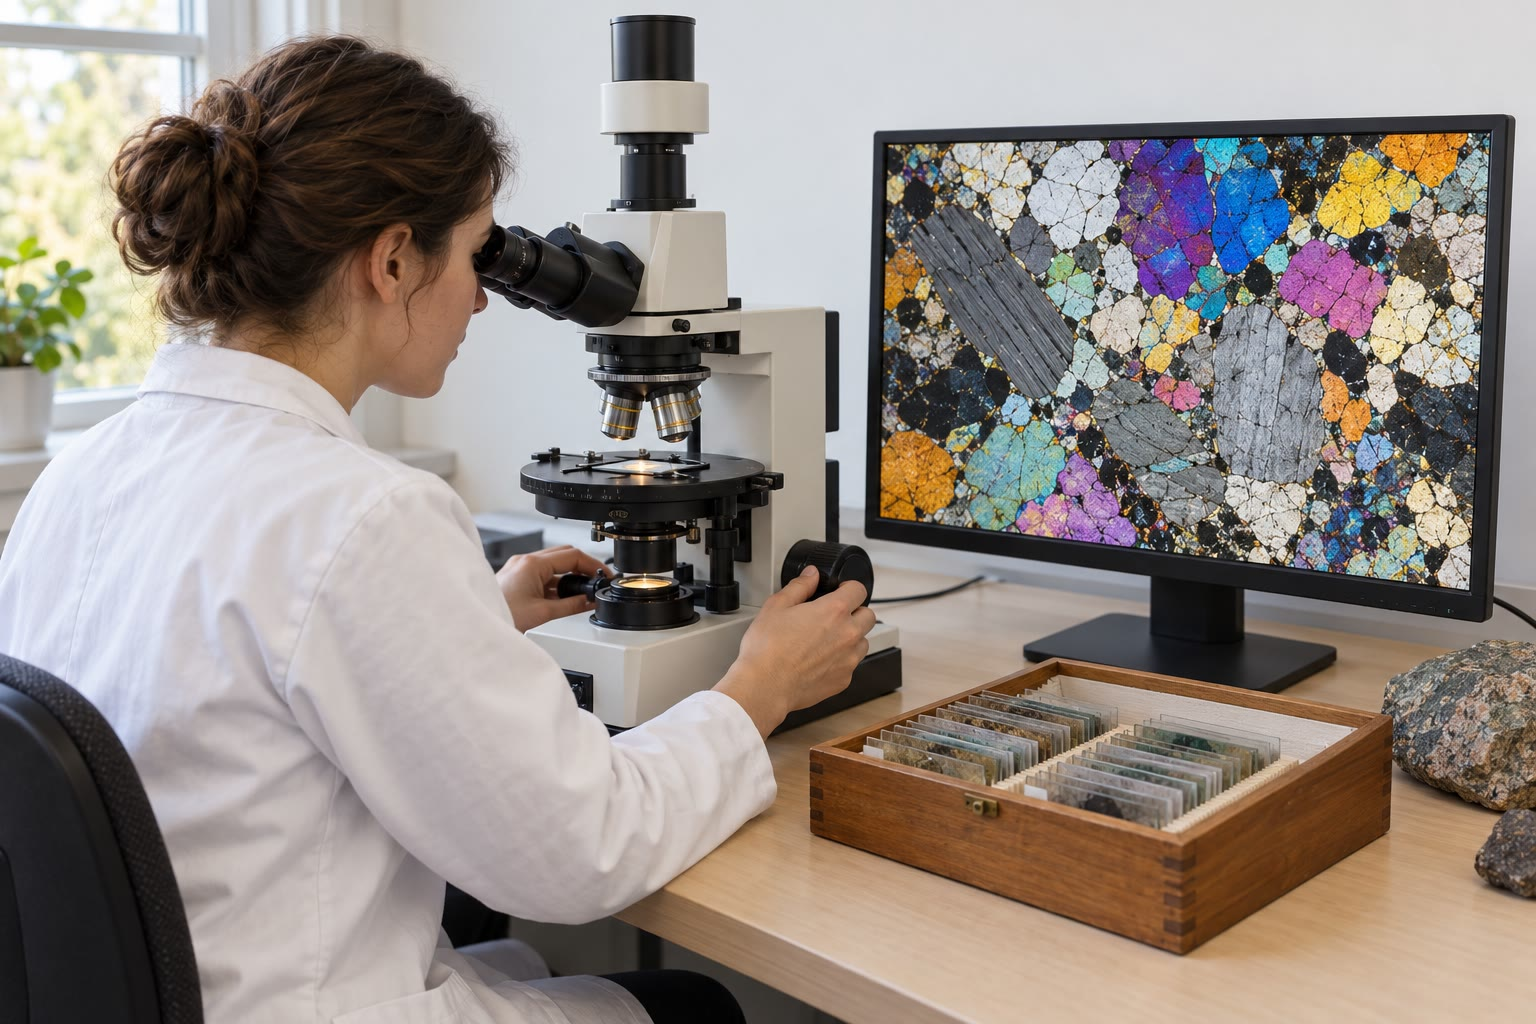
\includegraphics[width=\linewidth]{images/book5/ai/b3-petrology-desk.jpg}

{\scriptsize 岩石学家在偏光显微镜前工作，身旁是一盒薄片，
屏幕上显示偏振光下的一张薄片
（AI 生成插图）。}
\end{minipage}
\end{inthelab}

\section{练习}

\begin{exercise}[$\star$]\label{exo:b3:petrological-thermodynamics:1}
由表中数据，钠长石的 $\Delta_fH^\circ = \qty{-3935.0}{kJ}$，$S^\circ =
\qty{207.4}{J.K^{-1}}$，$V = \qty{100.07}{cm^3}$；硬玉 $-3029.3$，133.5，
60.40；石英 $-910.7$，41.5，22.69（均为每摩尔）。对于反应钠长石 = 硬玉 + 石英，
求 $\Delta_rH$、$\Delta_rS$、$\Delta_rV$（单位为 \unit{J.bar^{-1}}）、
克拉珀龙斜率，以及在 \qty{600}{\celsius} 时该线对应的压强，
并假定各性质为常数。
\end{exercise}
% ledger: rh95:ab-jd-qz

\begin{exercise}[$\star$]\label{exo:b3:petrological-thermodynamics:2}
一块属于 \ce{MgO}--\ce{SiO2} 体系的岩石含有镁橄榄石、顽火辉石和
石英。应用\omterm{prop:b3:petrological-thermodynamics:goldschmidt}{矿物相律}，并说明你的结论。
\end{exercise}

\begin{exercise}[$\star$]\label{exo:b3:petrological-thermodynamics:3}
求石榴子石中钙铝榴石和镁铝榴石的理想活度，该石榴子石中
$X_{\text{Ca}} = 0.20$，$X_{\text{Mg}} = 0.15$；并求斜长石中钙长石的理想活度，该斜长石中
$X_{\text{an}} = 0.40$（单一位置）。
\end{exercise}

\begin{exercise}[$\star$]\label{exo:b3:petrological-thermodynamics:4}
求正规溶液的临界温度，其中 $W =
\qty{15}{kJ.mol^{-1}}$。$W$ 为多少时 $T_c = \qty{1000}{K}$？
\end{exercise}

\begin{exercise}[$\star\star$]\label{exo:b3:petrological-thermodynamics:5}
在 \qty{1000}{K} 下，表中给出各物质的生成吉布斯能：
$-5432.2$（钙铝榴石）、$-3478.1$（钙长石）、$-2088.8$（蓝晶石）和 $-730.2$
（石英），单位为 \unit{kJ.mol^{-1}}。求 GASP 反应在
\qty{1}{bar} 下的 $\Delta_rG$ 及其平衡压强，并与实验线
$P_0 = 22.80\,T - 1093$（bar，\unit{\celsius}）作比较。
\end{exercise}
% ledger: rh95:gasp-ht, kn88:gasp

\begin{exercise}[$\star\star$]\label{exo:b3:petrological-thermodynamics:6}
对图中的正规溶液（$W = \qty{20}{kJ.mol^{-1}}$），求
$G_{\text{mix}}$ 在 $x = 0.5$、\qty{900}{K} 下的值，再求\omterm{def:b3:petrological-thermodynamics:solvus}{固溶线}分支 $x =
0.111$ 处的值。证明将成分为 0.5 的晶体分裂为两个分支
会降低其吉布斯能，并求降低的幅度。
\end{exercise}

\begin{exercise}[$\star\star$]\label{exo:b3:petrological-thermodynamics:7}
在三组分体系中，一个不变点处有多少个相交于此，有多少条
单变线从其发出？对图中的线束，
逐一检验四个反应是否均已配平。
\end{exercise}

\begin{exercise}[$\star\star$]\label{exo:b3:petrological-thermodynamics:8}
图中正规溶液中全岩成分为 $X_0 = 0.3$ 的一块岩石，
已冷却至 \qty{900}{K}，此时\omterm{def:b3:petrological-thermodynamics:solvus}{固溶线}分支分别为 0.111 和 0.889。
求各相所占的比例。
\end{exercise}

\begin{exercise}[$\star\star$]\label{exo:b3:petrological-thermodynamics:9}
利用 GASP 压力计 $P = P_0 + (3RT/6.21)\ln(X_{\text{Ca}}/X_{\text{an}})$
（bar），求在 \qty{900}{K} 时 $\partial P/\partial X_{\text{an}}$ 的值，
$X_{\text{an}} = 0.30$ 处的值。$X_{\text{an}}$ 有 0.01 的误差时，
压强会改变多少？
\end{exercise}

\begin{exercise}[$\star\star\star$]\label{exo:b3:petrological-thermodynamics:10}
证明正规溶液的旋节线满足 $x(1 - x) = RT/(2W)$。
当 $W = \qty{20}{kJ.mol^{-1}}$ 时，成分为 0.3 的晶体在何温度下
对任意微小涨落变得不稳定？将其与该晶体达到\omterm{def:b3:petrological-thermodynamics:solvus}{固溶线}时的温度
$T = W(1 - 2x)/[R\ln((1 - x)/x)]$ 相比较，
并解释两者之间的差距。
\end{exercise}

\begin{exercise}[$\star\star\star$]\label{exo:b3:petrological-thermodynamics:11}
证明对称正规溶液的\omterm{def:b3:petrological-thermodynamics:solvus}{固溶线}满足 $RT\ln[x/(1 -
x)] + W(1 - 2x) = 0$，并证明\omterm{def:b3:petrological-thermodynamics:solvus}{固溶线}的极大值 $T_c = W/(2R)$，在 $x
= 1/2$ 处取得。
\end{exercise}

\begin{exercise}[$\star\star\star$]\label{exo:b3:petrological-thermodynamics:12}
某岩石含有 \qty{2.0}{wt\percent} \ce{MnO}。含有
\qty{10}{wt\percent} \ce{MnO} 的石榴子石核心占岩石的 \qty{8}{wt\percent}，
且与基质相隔离。计算\omterm{def:b3:petrological-thermodynamics:pseudosection}{有效全岩成分}中的 \ce{MnO} 含量。
这一点对石榴子石边部的\omterm{def:b3:petrological-thermodynamics:pseudosection}{视剖面图}有何意义？
\end{exercise}

\section{问题：瓦尔登片岩的石榴子石}

\begin{problem}[{周末问题——一种虚构片岩的压强与温度，
依据数据表、相律、活度模型与
温压计求解}]
\label{pb:b3:petrological-thermodynamics:1}
% values: calc/ch11.py; gasp_tables.py
瓦尔登丘陵基底的片岩约在
\qty{480}{Ma} 前变质，含有石榴子石、黑云母、白云母、斜长石、蓝晶石和
石英。在石榴子石边部及其周围颗粒中，电子探针测得：
石榴子石 $X_{\text{Fe}} = 0.74$，$X_{\text{Mg}} = 0.12$，$X_{\text{Ca}} =
0.10$，$X_{\text{Mn}} = 0.04$；黑云母 $\ce{Mg}/(\ce{Mg} + \ce{Fe}) = 0.45$；
斜长石 $X_{\text{an}} = 0.30$。计算 GASP 反应时使用本章数据表，
温度计采用本科二年级分册中的公式
\[
T = \frac{52\,635 + 0.311P}{20.20 - 3R\ln K_D}\quad(T \text{ 以 K 计}, P
\text{ 以 bar 计}),
\]
及其实验地质压力计 $P = 22.80\,t - 1093 + (3RT/6.21)\ln
(X_{\text{Ca}}/X_{\text{an}})$，其中 $t$ 的单位为 \unit{\celsius}，$T$ 的单位为
开尔文。取 $R = \qty{8.314}{J.mol^{-1}.K^{-1}}$，地壳密度为
\qty{2800}{kg/m^3}，并取 $g = \qty{9.81}{m/s^2}$。

\medskip\noindent\textbf{第一部分——数据表。}
\begin{enumerate}
  \item 由汇总表计算 GASP 反应的 $\Delta_rH^\circ$、$\Delta_rS^\circ$
        以及 $\Delta_rV$。
  \item 计算 \qty{298.15}{K} 与 \qty{1}{bar} 下的 $\Delta_rG$。哪一侧在
        地表是稳定的？
  \item 在性质恒定的假设下，计算 \qty{900}{K} 时的端元压强，
        以及克拉珀龙斜率。
  \item 高温数据表给出 $\Delta_rG = \qty{81.5}{kJ}$，
        \qty{900}{K} 时为此值，\qty{1200}{K} 时为 \qty{119.8}{kJ}（\qty{1}{bar}）。
        计算相应压强。
  \item 与同一温度下的实验曲线进行比较。
  \item \qty{1200}{K} 时的差距需要 $\Delta_rH$ 有多大误差才能解释？
        与四个焓值的合成不确定度进行比较。
  \item 为什么热容的变化对结果影响如此之小？
\end{enumerate}

\medskip\noindent\textbf{第二部分——相律。}
\begin{enumerate}[resume]
  \item 列出描述六种矿物与一种水流体所需的组分，
        并统计相数。
  \item 用相律计算变度，
        并检验\omterm{prop:b3:petrological-thermodynamics:goldschmidt}{矿物相律}。
  \item 第二个样品中蓝晶石与夕线石并存，
        这说明其压强与温度有何特征？
  \item 变质作用过程中有水流经该岩石，
        这会如何改变计数结果？
\end{enumerate}

\medskip\noindent\textbf{第三部分——活度与温压计。}
\begin{enumerate}[resume]
  \item 计算钙铝榴石和钙长石的理想活度，
        以及岩石中 GASP 反应的 $\ln K$。
  \item 计算石榴子石–黑云母交换反应的 $K_D$。
  \item 计算 \qty{8}{kbar} 时的温度。
  \item 计算该温度下的 GASP 压强。
  \item 迭代求两个方程的交点。
  \item 用数据表中的端元直线代替实验直线，重新求两者的交点
        （取 $\Delta_rV = \qty{-6.61}{J.bar^{-1}}$）。
        你保留哪一个结果？为什么？
  \item 若 $X_{\text{an}}$ 有 0.05 的误差，
        结果会移动多少？
\end{enumerate}

\medskip\noindent\textbf{第四部分——埋藏过程。}
\begin{enumerate}[resume]
  \item 采用本科二年级分册中的恒定性质，蓝晶石 = 夕线石反应的
        $\Delta_rH = \qty{7.7}{kJ}$，$\Delta_rS =
        \qty{12.6}{J.K^{-1}}$，$\Delta_rV = \qty{0.571}{J.bar^{-1}}$。该结果是否位于
        蓝晶石稳定域内？
  \item 计算埋藏深度。
  \item 石榴子石核心的 $X_{\text{Ca}} = 0.07$，并与
        $X_{\text{an}}$ 相同的斜长石共同生长，温度大致相同。
        该核心形成于比边部更深还是更浅处？
  \item 给出瓦尔登片岩的峰值压强与埋藏深度。
\end{enumerate}
\end{problem}
